\documentclass{article}
\usepackage{tikz}
\usetikzlibrary{arrows}
\usepackage[pagebackref]{hyperref}

\begin{document}
\pagestyle{empty}
\noindent
\url{https://cecs.wright.edu/~pmateti/Courses/730/}
\section*{RPC Marshalling of Linked Data Structures}

%\subsection*{Signature of Function foo}
\begin{minipage}[t]{0.5\linewidth}
\begin{verbatim}
typedef struct List {
  int value;
  struct List * next;
} List;
\end{verbatim}
\end{minipage}
\quad
\begin{minipage}[t]{0.5\linewidth}
\begin{verbatim}
typedef struct Tree {
  int value;
  List * ptrtoint;
  struct Tree * left;
  struct Tree * right;
} Tree;
\end{verbatim}
\end{minipage}

\begin{verbatim}
foo(in List * a, in int b, in Tree * c, out float * d);
\end{verbatim}

\begin{figure}[h]\centering
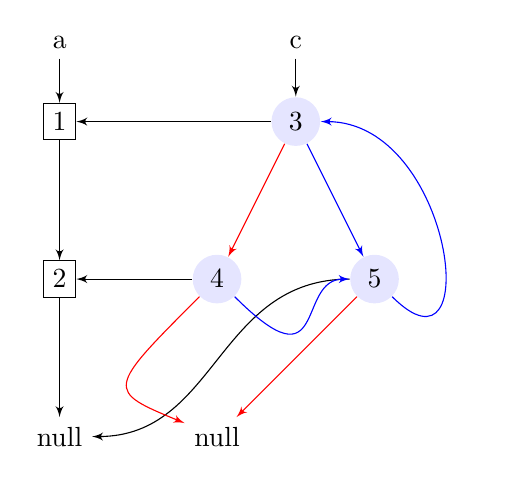
\begin{tikzpicture}[>=latex']
  \tikzstyle{tree}=[circle,fill=blue!10]
  \tikzstyle{square}=[rectangle,draw=black]


\begin{scope}
\node  (ca) at (3,7) {a};
\node [square] (c1) at (3,6) {1};
\node [square] (c2) at (3,4) {2};
\node (c0) at (3,2) {null};
\draw [->] (ca) -- (c1);
\draw [->] (c1) -- (c2);
\draw [->] (c2) -- (c0);

\node (cc) at (6,7) {c};
\node [tree] (c3) at (6,6) {3};
\node [tree] (c4) at (5,4) {4};
\node [tree] (c5) at (7,4) {5};
\node (c00) at (5,2) {null};
\draw [->] (c3) -- (c1);
\draw [->] (c4) -- (c2);
\draw [->] (c5) .. controls +(west:2cm) and +(right:2cm) .. (c0);

\draw [->] (cc) -- (c3);
\draw [->,red] (c3) -- (c4);
\draw [->,blue] (c3) -- (c5);
\draw [->,blue] (c4) .. controls +(south east:2cm) and +(left:1cm).. (c5);
\draw [->,red] (c4) .. controls +(south west:2cm) .. (c00);
\draw [->,blue] (c5) .. controls +(south east:2cm) and +(right:2cm) .. (c3);
\draw [->,red] (c5) .. controls +(south west:2cm) .. (c00);
\end{scope}
\end{tikzpicture}
\caption{Example Data Structure foo(a, b, c, d) [Must we have two null-s?]}
\end{figure}

\begin{figure}[h]\centering
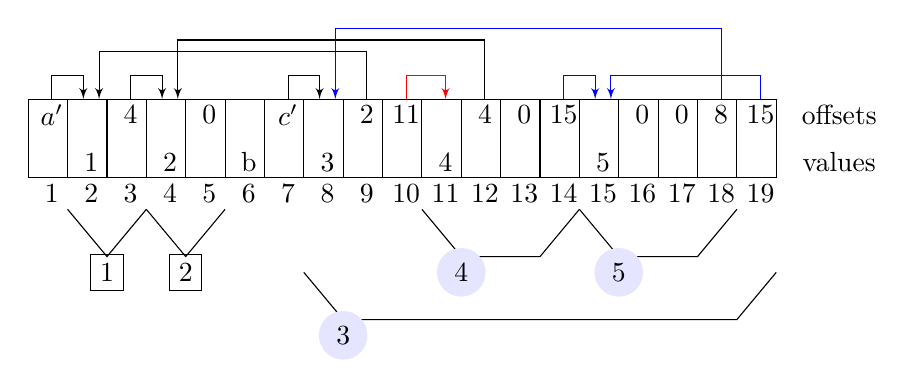
\begin{tikzpicture}[>=latex']
  \tikzstyle{tree}=[circle,fill=blue!10]
  \tikzstyle{square}=[rectangle,draw=black]

\begin{scope}
\draw (0, 0) -- (9.5, 0);
\draw (0,0) -- (0,1)  -- (9.5, 1);
\foreach \x in {1,2,...,19} {
  \draw (0.5*\x,0) -- (0.5*\x,1);
  \node at (0.5*\x - 0.2,-2mm) {\x};
}

\node at (0.5*21 - 0.2, 8mm) {offsets};
\foreach \x/\xtext in {1/$a'$, 2/, 3/4, 4/, 5/0, 6/, 7/$c'$, 8/, 9/2,
  10/11, 11/, 12/4, 13/0, 14/15, 15/, 16/0, 17/0, 18/8, 19/15} {
 \node at (0.5*\x - 0.2, 8mm) {\xtext}; 
}

\node at (0.5*21 - 0.2, 2mm) {values};
\foreach \x/\xtext in {1/, 2/1, 3/, 4/2, 5/, 6/b, 7/, 8/3, 9/, 10/,
  11/4, 12/, 13/, 14/, 15/5} {
  \node at (0.5*\x - 0.2, 2mm) {\xtext};
}

\newcommand{\aro}[4]{
  \draw [->,#4] (#1,1) -- (#1,1+#3) -- (#2,1+#3) -- (#2,1);
}

\foreach \a/\b/\h/\c in {1/1.8/1/, 3/3.8/1/, 7/7.8/1/, 10/11/1/red, 14/14.8/1/blue, 19/15.2/1/blue, 9/2.2/2/, 12/4.2/2.5/, 18/8.2/3/blue} {
  \aro{0.5*\a - 0.2}{0.5*\b - 0.2}{0.3*\h}{\c}
}

\newcommand{\brkt}[5]{
  \draw (0.5*#1 - 0.5,-4*#4mm) -- (0.5*#1,-4*#4mm-6mm) 
  -- (0.5*#2-0.5,-4*#4mm-6mm)  -- (0.5*#2,-4*#4mm);
  \node [#5] at (0.5*#1,-4*#4mm-8mm) {#3};
}

\foreach \a/\b/\t/\d/\n in {2/3/1/1/square, 4/5/2/1/square, 8/19/3/3/tree, 11/14/4/1/tree, 15/18/5/1/tree} {
  \brkt{\a}{\b}{\t}{\d}{\n}
}

\end{scope}
\end{tikzpicture}
\caption{DFS Marshalling the in-Parameters of foo}
\end{figure}



{\hfill
(Taken from a research paper.)}\\
\end{document}
